\documentclass{tufte-handout}
\usepackage{amsmath,amsthm}

\usepackage{pgfplots}
%\pgfplotsset{width=\textwidth,compat=1.5.1}

\newtheorem{claim}{Claim}[section]
\title{\sf Rainbow Perfect Matchings}
\author{Mats Rydberg \& Martin Larsson}

\begin{document}
\maketitle

\section{Algorithm}
\begin{enumerate}
\item Fix prime $p \gg n$ \sidenote{In our case, we selected $p = 32749$.}
\item For each colour $C \in [n]$
\subitem Construct $n \ast n$ matrix $m_C$
\subitem For each $uv \in E$ with $ c(uv) = C$
\subsubitem Pick random integer $r \in (0,p]$
\subsubitem Set $m_C[u,v] = r$
\item Set $B = \sum_{i = 0}^{n-1}m_i$
\item Compute $d_B =$ det$(B)$ mod $p$
\item If $d_B = 0$ return ''no''
\item Else set $sum = 0$
\item For each $X \subset [n]$
\subitem Initialize $M = \mathbf{0}$ \sidenote{$\mathbf{0}$ is the $n \ast n$ all-zeroes matrix.}
\subitem For each $C \in X$
\subsubitem Set $M = M + m_C$
\subitem Set $sum = sum + (-1)^{n-1-|X|} \cdot$ det$(M)$ mod $p$
\item If $d_B - sum = 0$ return ''no'' else return ''yes''
\end{enumerate}

\noindent Our algorithm modifies the given Algorithmic Piece 1 on step 2, by creating $n$ matrices, one for each colour. But in step 3 we combine them into the biadjacency matrix $B$ (called $A_G$ in the assignment) and do the same end condition for its determinant.

For Algorithmic Piece 2, we have modified the pseudo code to be defined via matrix sums instead. We construct the biadjacency matrix for the current set of colours by simple addition, and compute the determinant for every such matrix. We are not including det($B$) in $sum$, so to get the signs right we subtract an extra $1$ in the exponent for $-1$.\sidenote{Another way to fix this would be to compute $d_B + sum$ in step 7 of the algorithm, but we thought this was cleaner.} This is really just an optimization, as we could remove steps 3 and 4 and have Algorithmic Piece 2 more or less intact. Our algorithm is faster for ''no''-instances, however. With this change in mind, the logic is the same as in the assignment for why a non-rainbow perfect matching will eliminate itself in the calculation of $sum$.
\newpage





\section{Running Time}
\begin{enumerate}
\item $O(1)$
\item $O(n)$
\subitem $O(1)$
\subitem Worst case $n$ edges of colour $C$ from all $n$ nodes $\Rightarrow O(n^2)$
\subsubitem $O(1)$
\subsubitem $O(1)$
\item $T(n) = n^3$ additions. $\Rightarrow O(n^3)$
\item $O(1)$
\item $O(1)$
\item There are $2^n$ subsets to a set of $n$ elements $\Rightarrow T(n) = 2^n - 2\text{(the empty set and the full set)} \Rightarrow O(2^n)$
\subitem $O(1)$
\subitem Since $|X| \leq n-1$, this is $O(n)$, right?
\subsubitem $n^2$ additions $\Rightarrow O(n^2)$?
\subitem $T(n) = 1 + (n-2) + O(det(M))$
\item $O(1)$
\end{enumerate}


$$T(n) = 1 + n(1 + n^2(1 + 1)) + (n^3 | 1) + 1 + 1 + (2^n - 2)\cdot(1 + n(n^2 | 1) + 1 + (n - 2) + O(det(M))$$ 
$$ \leq 3 - n + n^3 - 2T(det(M)) + 2^n(n + n^3 + T(det(M)))$$
$$ \leq 2^n(n + n^3 + T(det(M)))$$

$$T(det(M)) = ?$$
The anwer will probably become
$$O(2^n)$$
eventually. But how do we convince ourselves?

I asked on Piazza.

\newpage
\section{Failure bound}



\begin{marginfigure}
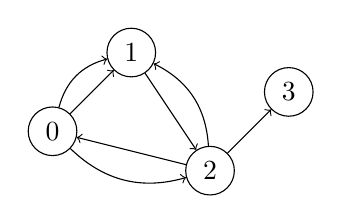
\begin{tikzpicture}
\node (0) [draw,circle] at (0,0) {0};
\node (1) [draw,circle] at (1,1) {1};
\node (2) [draw,circle] at (2,-.5) {2};
\node (3) [draw,circle] at (3,.5) {3};
\draw [->] (0) to [bend left] (1);
\draw [->] (0) to  (1);
\draw [->] (0) to [bend right] (2);
\draw [->] (1) to  (2);
\draw [->] (2) to  (0);
\draw [->] (2) to [bend right] (1);
\draw [->] (2) to (3);
\end{tikzpicture}
\caption{A directed multigraph.}
\end{marginfigure}

\section{Analysis}

\subsection{Lol}

The files are in the data directory are:
\begin{quotation}
\begin{description}
\item[three.txt] The 4-vertex graph from Fig.~1.
\end{description}
\end{quotation}

\section{Report part maybe}

\subsection{Transition probabilities}

The transition matrix for the graph described in three.txt
is\sidenote{Fill in the right values. Set $\alpha=\frac{85}{100}$.}
\begin{equation*}
P = 
\left(
\begin{array}{cccc}
1 & 6 & \pi & 1\\
1 & 1/e & -2  & \cdots\\
1 & 1 & 0 \\
\vdots
\end{array}
\right)\,,
\end{equation*}

\noindent text is text is text is text

\medskip
\begin{fullwidth}
\small
\begin{tabular}{lcccccccccc}
three.txt & 2 (36.6\%) & 1 (27.5\%) & 0 (18.4\%) & 3 (17.3\%) \\
tiny.txt & [\ldots] &\\
medium.txt &\\
wikipedia.txt & \\
p2p-Gnutella08-mod.txt &
\end{tabular}
\end{fullwidth}

\end{document}
